\section{Vektoren}

\textit{$\bullet$ Skalarprodukt} \\
\textit{$\cdot$ Matrixprodukt}

\subsection{Addition}

$\vec{a} + \vec{b} = \begin{bmatrix}
    a_1 \\
    a_2 \\
    a_n \\
\end{bmatrix} + \begin{bmatrix}
    b_1 \\
    b_2 \\
    b_n \\
\end{bmatrix} = \begin{bmatrix}
    a_1 + b_1 \\
    a_2 + b_2 \\
    a_n + b_n \\
\end{bmatrix}$

\subsection{Multiplikation mit Skalar}

$\lambda \vec{a} = \lambda\begin{bmatrix}
    a_1 \\
    a_2 \\
    a_n \\
\end{bmatrix} = \begin{bmatrix}
    \lambda a_1 \\
    \lambda a_2 \\
    \lambda a_n \\
\end{bmatrix}$ \\

\textit{$\lambda \in$ Skalar}

\subsection{Nullvektor}

$\vec{0} = \begin{bmatrix}
    0 \\
    0 \\
\end{bmatrix}$

\subsection{Vektorinverses}

$-\vec{a} = - \begin{bmatrix}
    a_1 \\
    a_2 \\
    a_n \\
\end{bmatrix} = \begin{bmatrix}
    -a_1 \\
    -a_2 \\
    -a_n \\
\end{bmatrix}$

\textit{Vektor mit negativen Komponenten}

\subsection{Vektoren Gleichheit}

$\vec{a} = \begin{bmatrix}
    3 \\
    2
\end{bmatrix} = \vec{b}$

\textit{Vektoren sind gleich, wenn Komponenten gleich}

\subsection{Skalarprodukt}

$\vec{a} \bullet \vec{b} = \begin{bmatrix}
    a_1 \\
    a_2 \\
    a_n
\end{bmatrix} \bullet \begin{bmatrix}
    b_1 \\
    b_2 \\
    b_n
\end{bmatrix} = a_1 b_1 + a_2 b_2 + \dots + a_n b_n$

\begin{tabular}{cc}
    \multirow{6}{*}{
        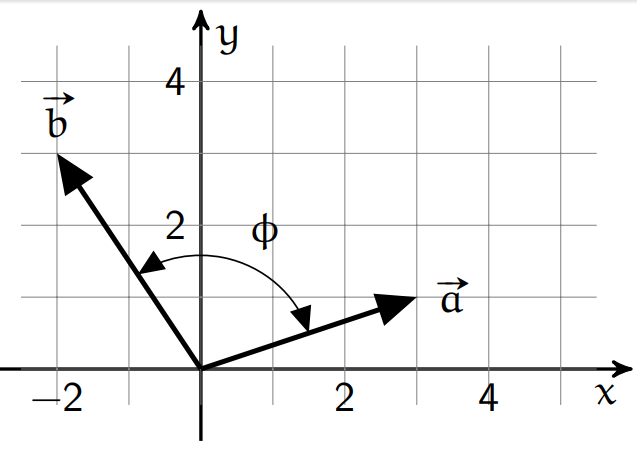
\includegraphics[width=0.25\textwidth]{assets/skaparprodukt.png}
    }
     & $\vec{a} \bullet \vec{b} = |\vec{a}| \cdot |\vec{b}| \cdot \cos \phi$ \\
     & \\
     & $|\vec{a}| = \sqrt{a_1^2 + a_2^2 + \dots + a_n^2}$ \\
     & $|\vec{b}| = \sqrt{b_1^2 + b_2^2 + \dots + b_n^2}$ \\
     & \\
     & $\cos \phi = \frac{\vec{a} \bullet \vec{b}}{|\vec{a}| \cdot |\vec{b}|}$ \\
\end{tabular}

\subsection{Skalarprodukt im beliebigem Koordinatensystem}

$\vec{a} = a_1\vec{e}_1 + a_2\vec{e}_2 + a_3\vec{e}_3 = [a_1 a_2 a_3]^T$ \\
$\vec{b} = b_1\vec{e}_1 + b_2\vec{e}_2 + b_3\vec{e}_3 = [b_1 b_2 b_3]^T$ \\

$\vec{a} \bullet \vec{b} = [a_1 a_2 a_3]\begin{bmatrix}
    g_{11} & g_{12} & g_{13} \\
    g_{21} & g_{22} & g_{23} \\
    g_{31} & g_{32} & g_{33} \\
\end{bmatrix} \begin{bmatrix}
    b_1 \\
    b_2 \\
    b_3
\end{bmatrix} = \mathbf{a}^T \mathbf{G} \mathbf{b}$

\textit{Matrix $\mathbf{G}$ wird \textbf{metrisch Tensor} genannt}

\subsection{Orthogonal}

$\vec{e}_x \bullet \vec{e}_y = 0$ \\
$\vec{a} \bullet \vec{b} = 0 \Leftrightarrow \vec{a} \bot \vec{b}$

\textit{
    Senkrecht zueinander, wenn Skalarprodukt zweier Einheitsvektoren 0 ergibt.
}

\subsection{Länge des Vektors}

$|\vec{a}| = \sqrt{\vec{a} \bullet \vec{a}} = \sqrt{a_1^2 + a_2^2 + \dots + a_n^2}$

\subsection{Einheitsvektor}

$ e_v = \frac{1}{\norm{v}} \bullet v = \frac{1}{\sqrt{v \cdot v}} \bullet v$ \\
$ ( i = e_1, j = e_2, k = e_3 ) $ \\

\textit{$\vec{e}_x = [1,0,0]^T$}\\
\textit{$\vec{e}_y = [0,1,0]^T$}\\
\textit{$\vec{e}_z = [0,0,1]^T$}

\subsection{Euklidische Distanz}

$\bar{AB} = \sqrt{(b_1-a_1)^2 + (b_2 - a_2)^2 + \dots + (b_n - a_n)^2}$

\subsection{Gerade im 2/3D}

\begin{itemize}
    \item \textbf{Punkt-Punktform mit Vektoren 2/3D} \\
          $\vec{r} = \vec{r}_1 + t(\vec{r}_1 - \vec{r}_0)$, $t \in \mathbb{R}$ \\
          $\vec{r}_1$: Punkt, $\vec{r}_2$: Punkt
    \item \textbf{Punkt-Richtungsform mit Vektoren 2/3D} \\
          $\vec{r} = \vec{r}_0 + t\vec{r}_1$, $t \in \mathbb{R}$ \\
          $\vec{r}_0$: Punkt, $\vec{r}_1$: Richtungsvektor
    \item \textbf{Achsenabschnitt-Steigungsform} \\
          $y=mx+b$ \\
          $b$: Achsenabschnitt, $m$: Steigung
    \item \textbf{Punkt-Richtungsform} \\
          $(y - y_0) = m(x - x_0)$ \\
          ($x_0$,$y_0$): Punkt, $m$: Steigung
    \item \textbf{Allgemeine Geradengleichung} \\
          $ax + by + c = 0$ \\
          $a,b,c \in \mathbb{R}$\\
    	  \\
    	  Aus Punkten A(x1, y1) und B(x2, y2) \\
    	  $\frac{y2 - y1}{x2 - x1} = \frac{y - y1}{x - x1}$
\end{itemize}

\subsection{Hessische Normalform}

\textit{Viktorielle Schreibweise der Hessischen Normalform}
\begin{tabular}{cl}
    \multirow{10}{*}{
        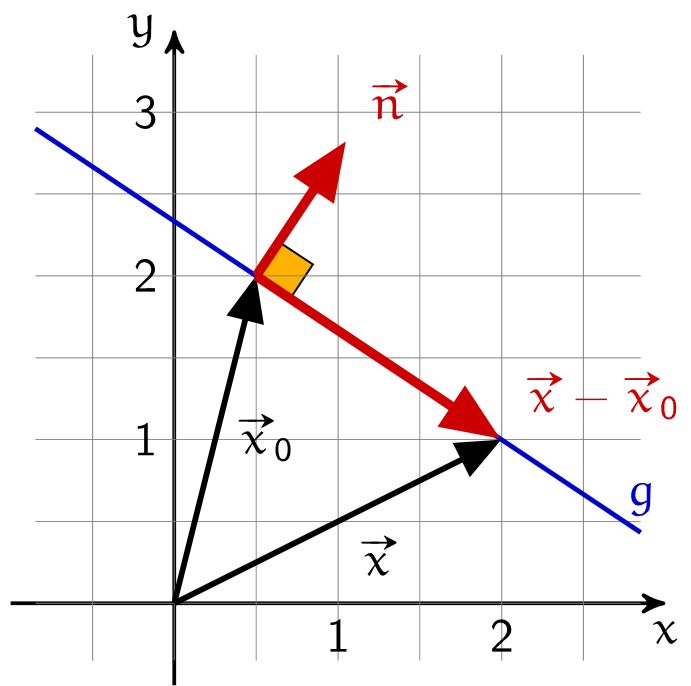
\includegraphics[width=0.2\textwidth]{assets/hessischenormalform.png}
    }
     & $\vec{n} \bullet (\vec{x} - \vec{x}_0) = 0$ \\
     & da $\vec{n} \bot (\vec{x} - \vec{x}_0)$ \\
     & $\Rightarrow n_x(x - x_0) + n_y(y - y_0) = $\\
     & $n_x x + n_y y - (n_x x_0 + n_y y_0)$\\
     & \\
     & Abstand vom Uhrsprung: $d$ \\
     & $d = (n_x x_0 + n_y y_0) = \vec{n} \bullet \vec{x}_0$\\
     & \\
     & \textit{$\vec{n}$ muss normalisiert sein:} \\
     & $|\vec{n}| = 1 \Rightarrow \frac{1}{\sqrt{n_x^2 + n_y^2}} \bullet \vec{n}$ \\
\end{tabular} \\

\begin{tabular}{cl}
    \multirow{10}{*}{
        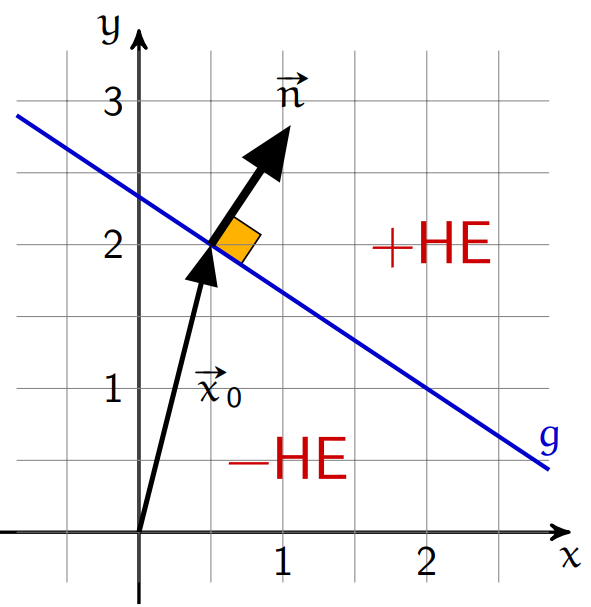
\includegraphics[width=0.2\textwidth]{assets/hessischenormalfromebene.png}
    }
     & $\mathbf{n_x x + n_y y - d = 0}$ \\
     & $d = (n_x x_0 + n_y y_0) = \vec{n} \bullet \vec{x}_0$\\
     & \\
     & $d > 0 \Leftrightarrow (0,0) \in -HE $ \\
     & $d < 0 \Leftrightarrow (0,0) \in +HE $ \\
     & \\
     & $g$: $ax + by + c = 0$\\
     & $\vec{n} = \begin{bmatrix}
         n_x \\
         n_y \\
     \end{bmatrix} = \frac{1}{\sqrt{a^2 + b^2}} \begin{bmatrix}
         a \\
         b \\
     \end{bmatrix}$ \\
     & $d = - \frac{c}{\sqrt{a^2 + b^2}}$ \\
     & \\
\end{tabular}

\subsection{Hessische Normalform Ebene}

$\epsilon: ax + by + cz + d = 0$ \\

$n_x x + n_y y + n_z z - D = 0$;
\textit{HNF der Ebene $\epsilon \in \mathbb{R}^3$}

$\vec{n} = \begin{bmatrix}
    n_x \\
    n_y \\
    n_z
\end{bmatrix} = \frac{1}{\sqrt{a^2 + b^2 + c^2}} \begin{bmatrix}
    a \\
    b \\
    c
\end{bmatrix} $ \\
$D = - \frac{d}{\sqrt{a^2 + b^2 + c^2}}$

\subsection{Achsenabschnitt}

\begin{tabular}{cl}
    \multirow{5}{*}{
        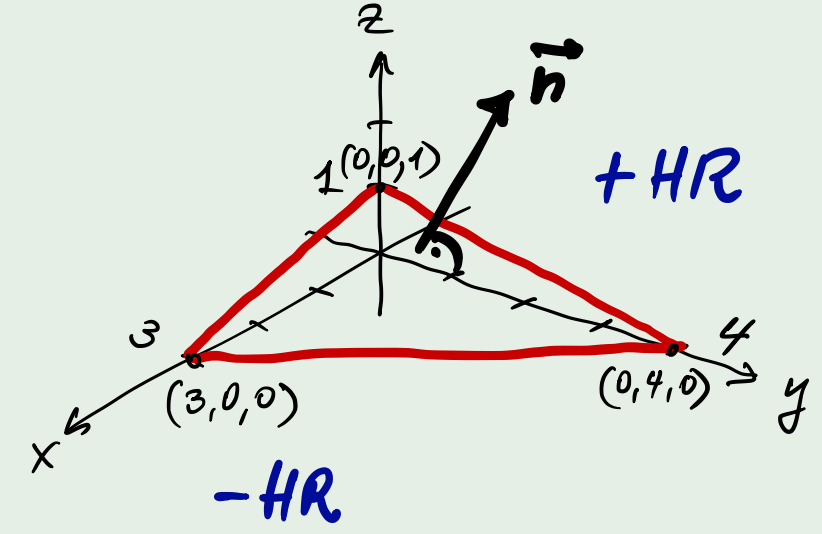
\includegraphics[width=0.2\textwidth]{assets/hnfachsenabschnitt.png}
    }
    & \textit{Gegeben sind 3 Punkte $p_x = x$, } \\
    & \textit{$p_y = y$, $p_z = z$ die ergeben eine } \\
    & \textit{Ebenegleichung:} \\
    & \\
    & $\mathbf{\frac{x}{p_x} + \frac{y}{p_y} + \frac{z}{p_z} - 1 = 0}$ \\
\end{tabular}

\subsection{Projektion eines Vektors}

\begin{tabular}{cl}
    \multirow{7}{*}{
        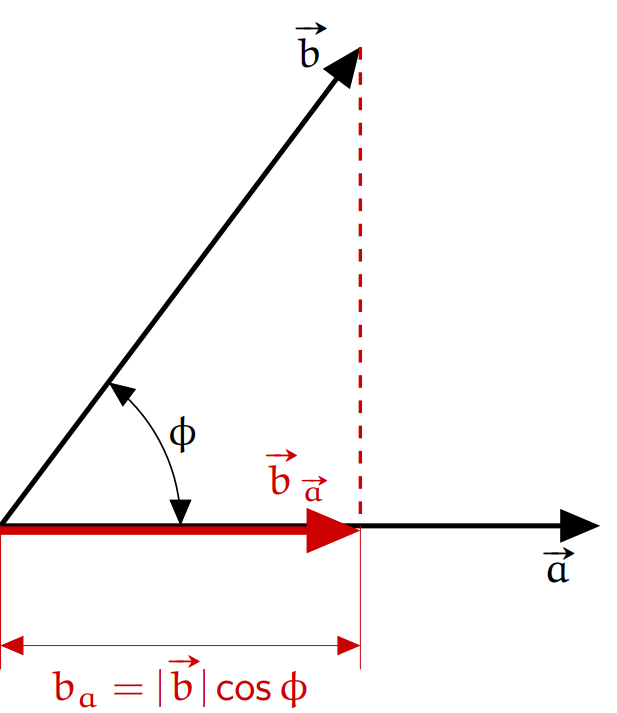
\includegraphics[width=0.15\textwidth]{assets/projection-of-vector.png}
    }
    & $\vec{b}$ Richtung $\vec{a}$:\\
    & $\vec{b}_{\vec{a}} = \frac{\vec{a} \bullet \vec{b}}{|\vec{a}|^2} \vec{a}$\\
    & \\
    & \textit{$b_a$ mal Einheitsvektor $\vec{a}$} \\
    &
        $\vec{b}_{\vec{a}} = b_a \frac{1}{|\vec{a}|} \vec{a} =
        |\vec{a}||\vec{b}|\cos \phi \frac{1}{|\vec{a}|} \vec{a}$ \\
    & $= \frac{\vec{a} \bullet \vec{b}}{|\vec{a}|^2} \vec{a}$\\
    & \\
\end{tabular}

\subsection{Vektorprodukt}

\begin{tabular}{cl}
    \multirow{7}{*}{
        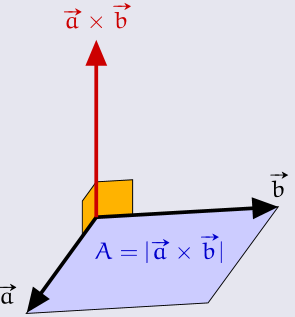
\includegraphics[width=0.15\textwidth]{assets/vectorproduct.png}
    }
    & $\vec{a} \times \vec{b}$ steht senkrecht auf beiden Vektoren \\
    & \\
    & $\vec{a}$, $\vec{b}$ und $\vec{a} \times \vec{b}$ sind ein Rechstsystem \\
    & \\
    & $\vec{a} \times \vec{b}$ entspricht der Fläche des \\
    & aufgespannten Parallelogramms ($A$): \\
\end{tabular} \\

$A = \sqrt{(a_2 b_3 - a_3 b_2)^2 + (a_3 b_1 - a_1 b_3)^2 + (a_1 b_2 - a_2 b_1)^2}$ \\

\begin{tabular}{cl}
    \multirow{4}{*}{
        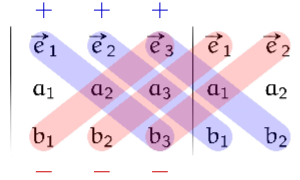
\includegraphics[width=0.15\textwidth]{assets/vectorproduct-build.png}
    }
    & $\vec{a} \times \vec{b} = \begin{bmatrix}
            \vec{e}_1 & \vec{e}_2 & \vec{e}_3 \\
            a_1 & a_2 & a_3 \\
            b_1 & b_2 & b_3 \\
        \end{bmatrix} = \begin{bmatrix}
            a_2 b_3 - a_3 b_2 \\
            a_3 b_1 - a_1 b_3 \\
            a_1 b_2 - a_2 b_1 \\
        \end{bmatrix}$ \\
    & $= (a_2 b_3 - a_3 b_2) \vec{e}_1 +$ \\
    & $(a_3 b_1 - a_1 b_3) \vec{e}_2 + (a_1 b_2 - a_2 b_1) \vec{e}_3 $ \\
\end{tabular} \\
\textit{Regel von Sarrus} \\

\subsection{Vektorprodukt Anwendung}

\begin{itemize}
    \item \textbf{Lorentz-Karft} $\vec{F} = q(\vec{v} \times \vec{B})$ \\
          $\vec{v}$: Geschwindigkeit, $B$: Magnetfeld, $q$: Landung
    \item \textbf{Geschwindigkeit} $\vec{v} = q(\vec{w} \times \vec{x})$ \\
          $\vec{x}$: Punkt, $w$: Winkelgeschwindigkeit, $\vec{w}$: Drehachse
    \item \textbf{Drehmoment} $\vec{M} = \vec{r} \times \vec{F}$ \\
          $\vec{F}$: Kraft, $\vec{r}$: Punkt / Koordinatenursprung
    \item \textbf{Normalvektor} $\vec{n} = \vec{a} \times \vec{b}$ \\
          $\vec{a}$ und $\vec{b}$ liegen auf der Ebene.
    \item \textbf{Kollinearität} kollinear (d.h. linear abhängig) wenn Vektorprodukt verschwinded
\end{itemize}

\subsection{Spatprodukt}

\begin{tabular}{cl}
    \multirow{6}{*}{
        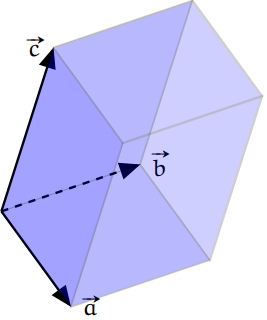
\includegraphics[width=0.12\textwidth]{assets/spatproduct.png}
    }
    & \textbf{Spatprodukt} $[\vec{a}, \vec{b}, \vec{c}]$ \\
    & \textit{Ist der Skalar der Vektoren $\vec{a}$, $\vec{b}$, $\vec{c}$} \\
    & \\
    & $[\vec{a}, \vec{b}, \vec{c}] = \vec{a} \bullet (\vec{b} \times \vec{c})$\\
    & \textit{Spatprodukt entsprich Volumen wenn in} \\
    & \textit{einem Rechstsystem, dann: $V_{Spat} = |[\vec{a}, \vec{b}, \vec{c}]|$} \\
\end{tabular} \\

$|[\vec{a}, \vec{b}, \vec{c}]| = $ \\
$a_1 b_2 c_3 + a_2 b_3 c_1 + a_3 b_1 c_2 - a_3 b_2 c_1 - a_1 b_3 c_2 - a_2 b_1 c_3$
\textit{Komplanar (linear abhängig) wenn $[\vec{a}, \vec{b}, \vec{c}] = 0$}

\subsection{Translation 2D}

$\vec{x}' = \vec{x} + \vec{t} = \begin{bmatrix}
    x_1 \\
    x_2 \\
\end{bmatrix} + \begin{bmatrix}
    t_1 \\
    t_2 \\
\end{bmatrix} = \begin{bmatrix}
    x_1 + t_1 \\
    x_2 + t_2 \\
\end{bmatrix}$

\subsection{Skalierung 2D}

$\vec{x}' = \begin{bmatrix}
    \vec{s}_x x \\
    \vec{s}_y y \\
\end{bmatrix} = \begin{bmatrix}
    s_x & 0 \\
    0 & s_y \\
\end{bmatrix} \begin{bmatrix}
    x \\
    y \\
\end{bmatrix}$

\subsection{Rotation 2D}

$\vec{x}' = \begin{bmatrix}
    x' \\
    y' \\
\end{bmatrix} = \begin{bmatrix}
    \cos(\phi) & -\sin(\phi) \\
    \sin(\phi) & \cos(\phi) \\
\end{bmatrix} \begin{bmatrix}
    x \\
    y \\
\end{bmatrix} = \mathbf{R}\vec{x}$

\textit{Inverse Matrix: $\mathbf{R}^{-1} = \mathbf{R}^T$}

\subsection{Vektor Rechenregeln}

\begin{tabular}{r|l}
    $\vec{a} + \vec{b} = \vec{b} + \vec{a}$ & Kommutativgesetz \\
    $\vec{a} + (\vec{b} + \vec{c}) = (\vec{a} + \vec{b}) + \vec{c}$ & Assoziativgesetz \\
    $\vec{a} + \vec{0} = \vec{a}$ & Existenz Neutralelement $\vec{0}$ \\
    $\vec{a} + (-\vec{a}) = \vec{0}$ & Existenz Inverses -$\vec{a}$ \\
    $\lambda(\vec{a} + \vec{b}) = \lambda \vec{a} + \lambda \vec{b}$ \\
    $(\lambda + \mu) \vec{a} = \lambda \vec{a} + \mu \vec{a}$ \\
    $(\lambda \mu) \vec{a} = \lambda(\mu \vec{a}) = \mu (\lambda \vec{a})$ \\
    $1 \vec{a} = \begin{bmatrix}
        1 \\
        1
    \end{bmatrix} \vec{a} = \vec{a}$

\end{tabular}

\subsection{Rechenregel Skalarprodukt}

$\vec{a} \bullet \vec{b} = \vec{b} \bullet \vec{a}$ \\
$\vec{a} \bullet (\vec{b} + \vec{c}) = \vec{a} \bullet \vec{b} + \vec{a} \bullet \vec{c}$ \\
$\lambda (\vec{a} \bullet \vec{b}) = (\lambda \vec{a}) \bullet \vec{b} = \vec{a} \bullet (\lambda \vec{b})$

\subsection{Vektorprodukt Rechenregeln}

\begin{tabular}{r|l}
    $\vec{a} \times \vec{b} = -\vec{b} \times \vec{a}$ & Anti-Kommutativgesetz \\
    $\vec{a} \times (\vec{b} + \vec{c}) = \vec{a} \times \vec{b} + \vec{a} \times \vec{c}$ & Distributivgesetz \\
    $\lambda (\vec{a} \times \vec{b}) = (\lambda \vec{a}) \times \vec{b} = \vec{a} \times (\lambda \vec{b})$
\end{tabular}

\subsection{Spatprodukt Rechenregeln}

\begin{tabular}{r|l}
    $[\vec{a}, \vec{b}, \vec{c}] = -[\vec{b}, \vec{a}, \vec{c}]$ & zwei Vekoren vertauschen \\
                                                                 & entspricht Vorzeichenwechsel \\
    $[\vec{a}, \vec{b}, \vec{c}] = [\vec{c}, \vec{a}, \vec{b}] $ & Zyklisches Vertauschen \\
                                                                 & keine Änderung \\
    $[\lambda \vec{a}, \mu \vec{b}, \nu \vec{c}] = \lambda\mu\nu[\vec{a}, \vec{b}, \vec{c}]$ & Multiplikation \\
    $[\vec{a} + \vec{b}, \vec{c}, \vec{d}] = $ & Addition \\
    $[\vec{a}, \vec{c}, \vec{d}] + [\vec{b}, \vec{c}, \vec{d}]$ & \\
\end{tabular}

\subsection{Begriffe}

\begin{tabular}{r|l}
    \textbf{Ortsvektor}         & Vom Ursprung zum Punkt \\
    \textbf{Richtungsvektor}    & Eine Richtung im Raum \\
    \textbf{Einheitsvektor}     & Eine Einheit in eine beliebige \\
                                & Richtung \\
    \textbf{Linearkombination}  & Ein Vektor, der ein vielfaches \\
    \textit{kollinear}          & eines Einheitvektors ist. \\
                                & $\vec{c} = \lambda\vec{a} + \mu \vec{b}$ \\
    \textbf{Linear Unabhängig}  & Vektoren sind unabhängig wenn \\
    \textit{komplanar}         & $\lambda_1 \vec{a}_1 + \lambda_2 \vec{a}_2 + \dots + \lambda_n \vec{a}_n = \vec{0}$ \\
                                & $\Leftrightarrow \lambda_1 = \lambda_2 = \dots = \lambda_n = 0$ \\
    \textbf{Skalar}             & Ist ein reelle oder komplexe Zahl \\
    \textbf{Rechtssystem}       & Koordinatensystem aufgebaut wie die \\
                                & rechte Hand wobei; der Zeigfinger \\
                                & X-Achse ($\vec{e}_x$), Mittelfinger \\
                                & Y-Achse ($\vec{e}_y$) und Daumen \\
                                & Z-Achse ($\vec{e}_z$) \\
\end{tabular}